\documentclass[12pt,a4paper]{article}

\usepackage[T1,T2A]{fontenc}
\usepackage[utf8]{inputenc}
\usepackage[english, russian]{babel}
\usepackage{indentfirst}
\usepackage{misccorr}
\usepackage{graphicx}
\usepackage{amsmath}
\usepackage{graphicx}
\usepackage{float}
\usepackage[left=20mm,right=10mm, top=20mm,bottom=20mm,bindingoffset=0mm]{geometry}

\setlength{\parskip}{6pt}
\DeclareGraphicsExtensions{.png}

\begin{document}

    \begin{titlepage}
        \begin{center}
            \large
            Санкт-Петербургский политехнический университет\\Петра Великого\\
            \vspace{0.5cm}
            Институт прикладной математики и механики\\
            \vspace{0.25cm}
            Кафедра «Прикладная математика»
            \vfill
            \textsc{\LARGE\textbf{Отчет по лабораторной работе №6}}\\[5mm]
            \Large
            по дисциплине\\"Математическая статистика"
        \end{center}
        \vfill
        \begin{tabular}{l p{175} l}
            Выполнила студентка\\группы 3630102/80201 && Деркаченко Анна Олеговна
            \vspace{0.25cm}
            \\Проверил\\доцент, к.ф.-м.н. && Баженов Александр Николаевич
        \end{tabular}
        \vfill
        \begin{center}
            Санкт-Петербург\\2021 г.
        \end{center}
    \end{titlepage}

\newpage
\begin{center}
    \tableofcontents
    \setcounter{page}{2}
\end{center}
\newpage
\begin{center}
    \listoffigures
\end{center}

\newpage
\section{Постановка задачи}
Дано нормальное двумерное распределение $N(x,y,0,0,1,1,\rho)$.

Необходимо:
\begin{enumerate}
    \item Найти оценки коэффициентов линейной регрессии $y_i=a+bx_i+e_i$, используя 20 точек на отрезке $[-1.8,2]$ с равномерным шагом, равным 0.2. Ошибку $e_i$ считать нормально распределенной с параметрами $(0,1)$
    \item В качестве эталонной зависимости взять $y_i=2+2x_i+e_i$
    \item При построении оценок коэффициентов использовать два критерия:
        \begin{itemize}
            \item критерий наименьших квадратов
            \item критерий наименьших модулей
        \end{itemize}
    \item Проделать те же действия для выборки, у которой в значения $y_1$ и $y_{20}$ вносятся возмущения 10 и -10
\end{enumerate}

\section{Теория}
\subsection{Простая линейная регрессия}
\subsubsection{Модель простой линейной регрессии}
\textit{Простая линейная регрессия} - регрессионная модель описания данных, такая что:
\begin{equation}
    y_i=\beta_0+\beta_1x_i+\varepsilon_i,i=\overline{1,n},
\end{equation}
где $x_1,...,x_n$ - заданные числа (значения фактора), $y_1,...y_n$ - наблюдаемые значения отклика, $\varepsilon_1,...,\varepsilon_n$ -  независимые, нормально распределенные $N(0,\sigma)$ с нулевым математическим ожиданием и одинаковой (неизвестной) дисперсией случайные величины (ненаблюдаемые),	$\beta_0,\beta_1$ - неизвестные параметры, подлежащие оцениванию.

Отклик $y$ зависит зависит от одного фактора $x$, и весь разброс экспериментальных точек объясняется только погрешностями наблюдений отклика $y$. Погрешности результатов измерений $x$ в этой модели полагают существенно меньшими погрешностей результатов измерений $y$, так что ими можно пренебречь.

\subsubsection{Метод наименьших квадратов}
В данном методе вводится мера (критерий) рассогласования отклика и регрессионной функции, и оценки параметров регрессии определяются так, чтобы сделать это рассогласование наименьшим. Используется критерий в виде суммы квадратов отклонений значений отклика от значений регрессионной функции (сумма квадратов остатков):
\begin{equation}
    Q(\beta_0,\beta_1)=\sum_{i=1}^n{\varepsilon_i^2}=\sum_{i=1}^n{(y_i-\beta_0-\beta_1x_i)^2}\rightarrow\min_{\beta_0,\beta_1}
\end{equation}

Расчётные формулы для МНК-оценок:
\begin{equation}
    \left\{
    \begin{array}{ll}
        \hat{\beta_1}=\frac{\bar{xy}-\bar{x}\cdot\bar{y}}{\bar{x^2}-(\bar{x})^2}\\
        \hat{\beta_0}=\bar{y}-\bar{x}\hat{\beta_1}
    \end{array}
    \right.
\end{equation}

\subsection{Робастные оценки коэффициентов линейной регрессии}
\textit{Робастность} оценок коэффициентов линейной регрессии - их устойчивость по отношению к наличию в данных редких, но больших по величине выбросов. Она может быть обеспечена использованием метода наименьших модулей вместо метода наименьших квадратов:
\begin{equation}
    \sum_{i=1}^n{|y_i-\beta_0-\beta_1x_i|}\rightarrow\min_{\beta_0,\beta_1}
\end{equation}

Робастная альтернатива оценкам коэффициентов линейной регрессии по МНК:
\begin{equation}
    \left\{
    \begin{array}{ll}
        \hat{\beta_1}_R=r_Q\frac{q^*_y}{q^*_x}\\
        \hat{\beta_0}_R=medy-\hat{\beta_1}_R medx
    \end{array}
    \right.
\end{equation}
где $med x$ и $med y$ - робастные выборочные медианы, $q^*_x$ и $q^*_y$ - робастные нормированные интерквартильные широты, $r_Q$ - знаковый коэффициент корреляции. Причем:
\begin{equation}
    \left\{
    \begin{array}{ll}
        r_Q=\frac{1}{n}\sum_{i=1}^n{sgn(x_i-medx)sgn(y_i-medy)}\\
        q^*_x=\frac{x_j-x_l}{k_q(n)}\\
        q^*_y=\frac{y_j-y_l}{k_q(n)}\\
        l=\begin{cases}
                [\frac{n}{4}]+1\text{ при }\frac{n}{4}\text{ - дробном}\\ 
                \frac{n}{4}\text{ при }\frac{n}{4}\text{ - целом}
            \end{cases}\\
        j=n-l+1
    \end{array}
    \right.
\end{equation}

Уравнение регрессии принимает вид:
\begin{equation}
    y=\hat{\beta_0}_R+\hat{\beta_1}_Rx
\end{equation}

\section{Реализация}
Реализация лабораторной работы проводилась на языке Python в среде разработки PyCharm c использованием дополнительных библиотек:
\begin{itemize}
    \item scipy
    \item numpy
    \item matplotlib
\end{itemize}

Исходный код лабораторной работы размещен в GitHub-репозитории.

URL: https://github.com/derkanw/Mathstat/tree/main/lab6

\section {Результаты}
\subsection{Выборка без возмущения}
Оценка коэффициентов по критерию наименьших квадратов:
\begin{equation}
    \left\{
    \begin{array}{ll}
        \hat{\beta_0}=2.198856\\
        \hat{\beta_1}=1.942401
    \end{array}
    \right.
\end{equation}

Удаленность по мере в пространстве $l^2:0.826971$

Оценка коэффициентов по критерию наименьших модулей:
\begin{equation}
    \left\{
    \begin{array}{ll}
        \hat{\beta_0}_R=2.154839\\
        \hat{\beta_1}_R=1.947938
    \end{array}
    \right.
\end{equation}

Удаленность по мере в пространстве $l^1: 2.941948$
\begin{figure}[H]
    \centering
    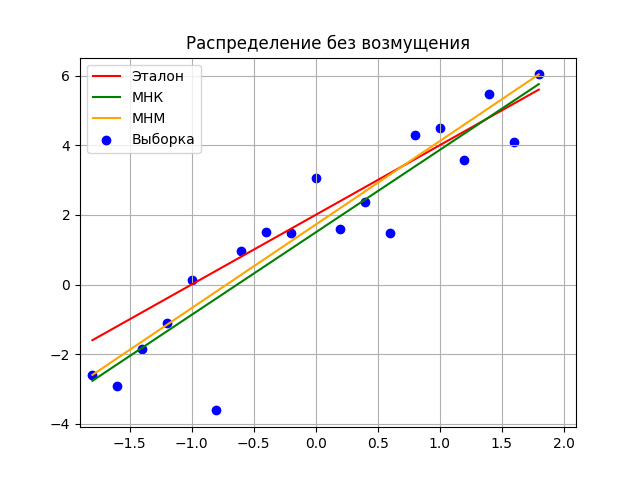
\includegraphics{images/noDisturbance.png}
    \caption{Выборка из 20 элементов без возмущения}
\end{figure}

\subsection{Выборка с возмущением}
Оценка коэффициентов по критерию наименьших квадратов:
\begin{equation}
    \left\{
    \begin{array}{ll}
        \hat{\beta_0}=2.198856\\
        \hat{\beta_1}=0.363454
    \end{array}
    \right.
\end{equation}

Удаленность по мере в пространстве $l^2:61.816189$

Оценка коэффициентов по критерию наименьших модулей:
\begin{equation}
    \left\{
    \begin{array}{ll}
        \hat{\beta_0}_R=2.316183\\
        \hat{\beta_1}_R=1.440918
    \end{array}
    \right.
\end{equation}

Удаленность по мере в пространстве $l^1:10.97349$
\begin{figure}[H]
    \centering
    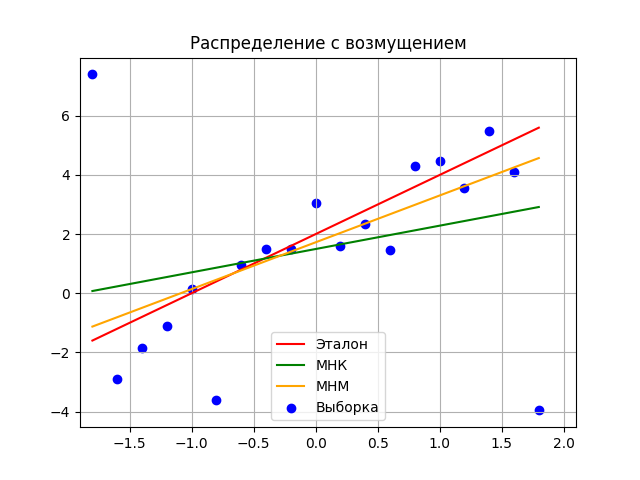
\includegraphics{images/disturbance.png}
    \caption{Выборка из 20 элементов с возмущением}
\end{figure}

\section{Обсуждение}
Метод наименьших квадратов и наименьших модулей работают в разный пространствах: в $l^2$ и в $l^1$ соответственно. Поэтому удаленность экспериментально построенной прямой от эталонной стоит рассматривать только в контексте каждого из пространств.

В ходе исследования полученный результатов можно сделать вывод, что метод наименьших квадратов дает более точную оценку коэффициентов линейной регрессии, но менее пригоден при выборке с редкими возмущениями достаточной величины. То есть метод наименьших модулей менее точен, но более устойчив, так как использует робастные величины.
\end{document}
